\chapter{Computations}\label{computations}
This chapter is dedicated to computations of rendezvous values for various spaces and related results.

We begin with an easy example
\begin{example}
	Consider the $m$-dimensional closed Ball $B:=\overline{B(O,\frac{1}{2})}$ with center at $O$ and radius $\frac{1}{2}$ in Euclidean $m$-space. Clearly $B$ is a compact connected Hausdorff space, therefore the Gross-Stadje-Theorem (\autoref{thm:gross-stadje})
	is applicable and there exists a unique rendezvous value $a(B,d)$ where $d$ is the usual Euclidean metric.
	
	Firstly, let us examine the case of $n=1$ and $x_1=O$. In this situation it is apparent that the rendezvous value is at most $\frac{1}{2}$.
	
	Secondly, consider the case $n=2$ with $x_1,x_2\in \partial B$ being antipodal points. Note that $d(x_1,x_2)=1$ and by triangle inequality we have for all $y\in B$:
	\[
	1=d(x_1,x_2)\leq d(x_1,y)+d(x_2,y)
	\]
	Multiplying both sides with $\frac{1}{2}$ gives
	\[
	\frac{1}{2}\leq a(B,d).
	\]
	Together with the previous result we conclude:
	\[
	a(B,d)\leq\frac{1}{2}\leq a(B,d)\quad \Rightarrow\quad a(B,d)=\frac{1}{2}
	\]
\end{example}

The following example can also be found in \cite{cleary:numbers-of-shapes}. The methods used here can be applied for many spaces.
\begin{example}
	Let $X\subset \mathbb{R}^2$ be an equilateral triangle (the $1$-dimensional polygon) with side length $\ell$ (with the usual subspace topology) and let $d$ be the Euclidean metric as before.
	
	
	\begin{centering}
		
		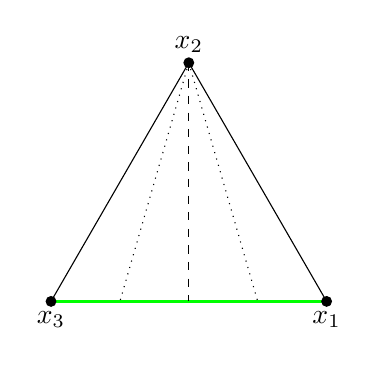
\begin{tikzpicture}[scale=3.5]
		\draw (1,0) node[below]{$x_1$}--(0,0) node[below]{$x_3$} -- +(60:1) node[above]{$x_2$}--cycle;
		\draw[very thick,green](0,0)--(1,0);
		\draw[dashed] (60:1)--(0.5,0);
		\draw[dotted] (60:1)--(0.25,0);
		\draw[dotted] (60:1)--(0.75,0);
		\filldraw (1,0) circle (0.5pt);
		\filldraw (0,0) circle (0.5pt);
		\filldraw (60:1) circle (0.5pt);
		\end{tikzpicture} 
		
	\end{centering}

First, consider the case $n=3$ and let $x_1,x_2,x_3$ be the vertices of the triangle.	By  symmetry we can assume that $y$ is contained in the edge between $x_1$ and $x_3$ (here marked green). It is easily verified that $d(x_1,y)+d(x_3,y)$ is independent from $y$ as long as it is contained in the edge joining those two vertices. Furthermore, it is clear, that the minimum of $d(x_2,y)$ is obtained for $y^\prime=(0.5,0)$. We therefore find:
	\[
	a(X,d)\geq \frac{1}{3}\cdot(d(x_1,y^\prime)+d(x_2,y^\prime)+d(x_3,y^\prime))=\frac{\ell}{3}\cdot \left(\frac{1}{2}+\sin\left(\frac{\pi}{3}\right)+\frac{1}{2}\right)=\ell\left(\frac{2+\sqrt{3}}{6}\right).
	\]
	
	Now, consider the case $n=3$ where $x_1,x_2,x_3$ are the midpoints of the edges.
	\begin{centering}
		
		
		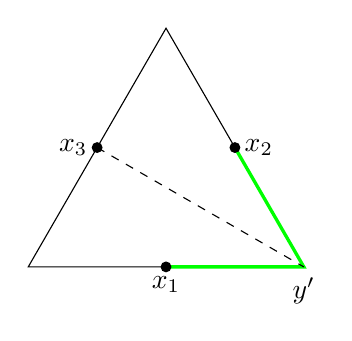
\begin{tikzpicture}[scale=3.5]
		\draw (1,0)--(0,0) -- +(60:1)--cycle;
		\draw[very thick,green](0.5,0)--(1,0) node[black,below]{$y^\prime$}-- +(120:0.5);
		\filldraw  (0.5,0) circle (0.5pt) node[below]{$x_1$};
		\filldraw (1,0)+(120:0.5) circle (0.5pt) node[right]{$x_2$};
		\filldraw (60:0.5) circle (0.5pt) node[left]{$x_3$};		
		\draw[dashed] (60:0.5)--(1,0);
		\end{tikzpicture}
		
	\end{centering}
	
	Again, by symmetry we see that we can restrict $y$ to be the "corner" between $x_1$ and $x_2$ (marked green again). It is easy to see that the vertex between $x_1$ and $x_2$ , denoted by $y^\prime$ from here on, is the point that is the furthest away from $x_1,x_2$ and $x_3$ simultaneously. Therefore, we find
	\[
	a(X,d)\leq \frac{\ell}{3}(d(x_1,y^\prime)+d(x_2,y^\prime)+d(x_3,y^\prime))=\frac{\ell}{3}\left(\frac{1}{2}+\frac{1}{2}+\sin\left(\frac{\pi}{3}\right)\right)=\ell\cdot \left(\frac{2+\sqrt{3}}{6}\right).
	\]
	With above result we see that equality holds.
\end{example}	
%	According to %todo ref
%	a similar method yields the following formula for a regular $n$-gon $X_n$ in $\mathbb{R}^2$:
%	\begin{align*}
%	a(X_n,d)&=\frac{1}{2n}\sum_{k=0}^{n-1}\left[\frac{3}{2}+\frac{1}{2}\cos\left(\frac{2\pi}{n}\right)-\cos\left(\frac{2k\pi}{n}\right)-\cos\left(\frac{2(k-1)\pi}{n}\right)\right]^{\frac{1}{2}}& \text{,when }n \text{ even}
%	\\
%	a(X_n,d)&=\frac{1}{n}\sum_{k=0}^{n-1}\left[\frac{\frac{3}{2}+\frac{1}{2}\cos\left(\frac{2\pi}{n}\right)-\cos\left(\frac{2k\pi}{n}\right)-\cos\left(\frac{2(k-1)\pi}{n}\right)}{2-2\cos\left(\frac{(n-1)\pi}{n}\right)}\right]^{\frac{1}{2}}& \text{,when }n \text{ odd}
%	\end{align*}

According to Cleary, Morris and Yost \cite{cleary:numbers-of-shapes}, Cleary computed the rendezvous value for regular $n$-gons in euclidean $2$-space with diameter $1$ to be 
	\begin{align*}
	a(X_n,d)&=\frac{1}{2n}\sum_{k=0}^{n-1}\left[\frac{3}{2}+\frac{1}{2}\cos\left(\frac{2\pi}{n}\right)-\cos\left(\frac{2k\pi}{n}\right)-\cos\left(\frac{2(k-1)\pi}{n}\right)\right]^{\frac{1}{2}}& \text{,when }n \text{ even}
	\\
	a(X_n,d)&=\frac{1}{n}\sum_{k=0}^{n-1}\left[\frac{\frac{3}{2}+\frac{1}{2}\cos\left(\frac{2\pi}{n}\right)-\cos\left(\frac{2k\pi}{n}\right)-\cos\left(\frac{2(k-1)\pi}{n}\right)}{2-2\cos\left(\frac{(n-1)\pi}{n}\right)}\right]^{\frac{1}{2}}& \text{,when }n \text{ odd}
	\end{align*}
	
Unfortunately, the original paper seems to have been lost, according to the La Trobe University Library (private communication).

However, a similar computation can be included in this paper from which Cleary's result follows easily:
%\newpage
\begin{example}
	Let $X_n$ be the regular $n$-gon in euclidean $2$-space with vertices on the unit circle. Consider the case $k=n$ and $x_i$ being the vertices of the $n$-gon.
	
	\begin{centering}
		\parbox{.5\linewidth}{
	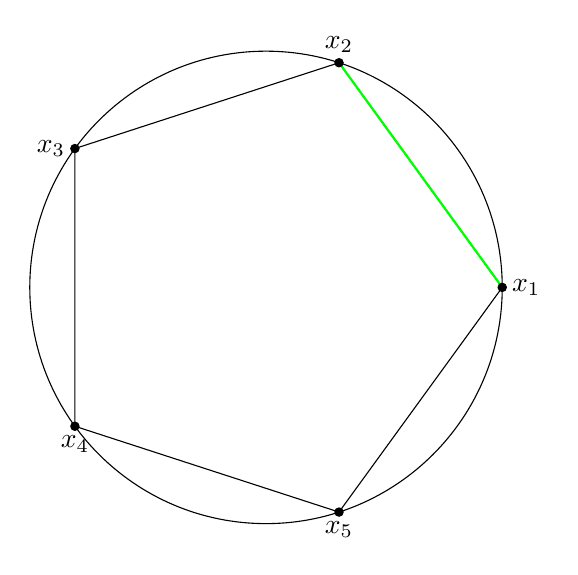
\begin{tikzpicture}[scale=3]
	\draw (0,0)+(0:1)node[right]{$x_1$} --+(72:1)node[above]{$x_2$}--+(144:1)node[left]{$x_3$}--+(-144:1)node[below]{$x_4$}--+(-72:1)node[below]{$x_5$}--cycle;
	\draw (0,0) circle(1);
	\draw[thick,green](0,0)+(72:1)--(1,0);
	\filldraw (1,0) circle (.5pt);
	\filldraw (72:1) circle (.5pt);
	\filldraw (144:1) circle (.5pt);
	\filldraw (216:1) circle (.5pt);
	\filldraw (288:1) circle (.5pt);
	\end{tikzpicture}}%
		\parbox{.5\linewidth}{
	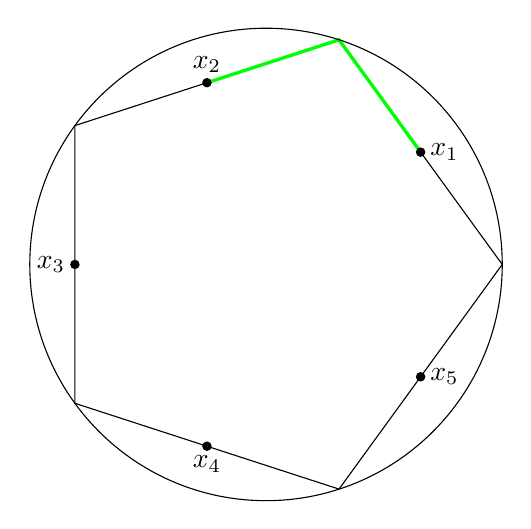
\begin{tikzpicture}[scale=3]
	\draw (0,0)+(0:1) --+(72:1)node[midway,right]{$x_1$}--+(144:1)node[midway,above]{$x_2$}--+(-144:1)node[midway,left]{$x_3$}--+(-72:1)node[midway, below]{$x_4$}--(1,0) node[midway,right]{$x_5$};
	\draw[green, very thick] (36:0.80902)--(72:1)--(108:0.80902);
	\filldraw (36:0.80902) circle (0.5pt);
	\filldraw (108:0.80902) circle (0.5pt);
	\filldraw (180:0.80902) circle (0.5pt);
	\filldraw (252:0.80902) circle (0.5pt);
	\filldraw (324:0.80902) circle (0.5pt);
	\draw (0,0) circle(1);
	\end{tikzpicture}
	}
	
	\end{centering}
Similar to the example of the equilateral triangle, we can restrict $y$ to be on the edge connecting $x_1$ and $x_2$. Evidently, 
\[
\frac{1}{k}\sum_{i=1}^k d(x_i,y)
\]
is minimized, if $y$ is the midpoint of this edge. By identifying $\R^2$ with $\C$ we find that this minimizer is given by \[y_{min}=\frac{1}{2}(\zeta_n+1),\] where $\zeta_n=\exp\left(\frac{2\pi i}{n}\right)$ is the $n$-th root of unity in $\C$. We find that
\newcommand{\zetan}{\exp\left(\frac{2\pi i}{n}\right)}
\newcommand{\zetanj}{\exp\left(\frac{2\pi i j}{n}\right)}
\newcommand{\zetancc}{\exp\left(\frac{2\pi i}{n}\right)}
\newcommand{\zetanjcc}{\exp\left(\frac{2\pi i j}{n}\right)}
\begin{align*}
\frac{1}{n}\sum_{j=1}^n d(x_j,y)&\leq \frac{1}{n}\sum_{j=1}^n \left|\frac{1}{2}(\zeta_n+1)-\zeta_n^j\right|=\frac{1}{n}\sum_{j=1}^n \left|\frac{1}{2}(\exp\left(\frac{2\pi i}{n}\right)+1)-\exp\left(\frac{2\pi i j}{n}\right)\right|
\\
&=\frac{1}{n}\sum_{j=1}^n \bigg[\bigg(\frac{1}{2}\bigg(1+\zetan\bigg)-\zetanj\bigg)\cdot
	\\&\hspace{2cm}\cdot
	\left(\frac{1}{2}\left(1+\zetancc\right)-\zetanjcc\right)\bigg]^{\frac{1}{2}}
\\
&=\frac{1}{n}\sum_{j=1}^n\bigg[\frac{1}{4}\left(1+\zetan\right)\left(1+\zetancc\right)
	\\&\hspace{2cm}
	-\frac{1}{2}\left(1+\zetan\right)\zetanjcc
	\\&\hspace{2cm}
	-\frac{1}{2}\zetan\left(1+\zetanjcc\right)+1\bigg]^{\frac{1}{2}}
\end{align*}
\begin{align*}
	\hspace{1cm}&=\frac{1}{n}\sum_{j=1}^n\bigg[\frac{1}{4}\left(2+2\cos\left(\frac{2\pi}{n}\right)\right)-\frac{1}{2}\zetancc
	\\
	&\hspace{2cm}-\frac{1}{2}\exp\left(\frac{2\pi i (j-1)}{n}\right)-\frac{1}{2}\zetanj
	%\\&\hspace{2cm}
	-\frac{1}{2}\exp\left(\frac{2\pi i(j-1)}{n}\right)+1\bigg]^{\frac{1}{2}}
\\
&=\frac{1}{n}\sum_{j=1}^n\bigg[\frac{3}{2}+\frac{\cos\left(\frac{2\pi}{n}\right)}{2}-\cos\left(\frac{2\pi j}{n}\right)-\cos(\frac{2\pi(j-1)}{n})\bigg]^{\frac{1}{2}}:=\alpha.
\end{align*}

To find a upper bound for $a(X_n,d)$, consider the case of $k=n$ and $x_j$ being the midpoints of the edges. It is easy to see that we would need to compute the same distances again, thus we can conclude that
\[
\alpha\geq \frac{1}{n}\sum_{j=1}^k d(x_j,y),
\]
yielding
\[
a(X_n,d)=\alpha.
\]
\end{example}


Morris and Nickolas \cite{Morris1983} found the following method for computing the rendezvous number:

\begin{theorem}
	Let $(X,d)$ be a compact, connected, non-empty metric space. If there is a Borel probability measure $\mu_0$ on $X$ such that the integral $\int_X d(x,y)\mu_0(\dx)$ is independent of the choice of $y\in X$, then the rendezvous number $a(X,d)$ is equal to $\int_X d(x,y)\mu_0(\dx)$ for any  $y\in X$.
\end{theorem}

\begin{proof}
	Fix one element $e$ in $X$ and let $\nu\in \M^1(X)$ be arbitrary. Then
	\begin{align*}
		\int_X\int_X d(x,y)\nu(\dy)\mu_0(\dx)&=\int_X\int_X d(x,y)\mu_0(\dx)\nu(\dy)
		\\
		&=\int_X\int_X d(x,e)\mu_0(\dx)\nu(\dy)
		\\
		&=\left(\int_X d(x,e)\mu_0(\dx)\right)\cdot\left(\int_X\nu(\dy)\right)
		\\
		&=\int_Xd(x,e)\mu_0(\dx).
	\end{align*}
	
	Since $\nu\in \M^1$ was arbitrary and $d$ is symmetric, this immediately implies that for any $\mu\in \M^1(X)$
	\[
	\int_X d(x,e)=\int_X\int_X d(x,y)\mu(\dx)\mu_0(\dy)\geq\inf\limits_{\nu\in \M^1}\int_X\int_X d(x,y)\mu(\dx)\nu(\dy).
	\]
	Thus,
	\[
	\sup_{\mu\in\M^1}\inf_{\nu\in\M^1}\int_X\int_X d(x,y)\mu(\dx)\nu(\dy)\leq\int_Xd(x,e)\mu_0(\dx).
	\]
	
	However, by our previous calculation,
	\begin{align*}
	\int_X d(x,e)\mu_0(\dx)=&\inf_{\mu\in\M^1}\int_X\int_X d(x,y)\mu_0(\dx)\nu(\dy)
	\\
	\leq&\sup_{\mu\in\M^1}\inf_{\nu\in\M^1}\int_X\int_X d(x,y)\mu(\dx)\nu(\dy).
	\end{align*}
	We conclude,
	\[
	\int_Xd(x,e)\mu_0(\dx)=\sup_{\mu\in\M^1}\inf_{\nu\in\M^1}\int_X\int_X d(x,y)\mu(\dx)\nu(\dy)=a(X,d).\qedhere
	\]
\end{proof}

Before we continue with a closely related result, we will use this statement to compute the rendezvous value of the circle as described by Morris and Nickolas \cite{Morris1983}.
\begin{example}
	Let $X\subset \R^2$ be a $1$-sphere with unite diameter and center at the origin. Let $\mu_0$ be the normed Lebesgue-measure. Then it is clear that $\int_X d(x,y)\mu_0(\dx)$ does not depend on the choice of $y$ by symmetry of the sphere. Thus, we may choose $y=\left(\frac{1}{2},0\right)$. We can express every point in $X$ as $x=\left(\frac{1}{2}\cos(\Theta),\frac{1}{2}\sin(\Theta)\right)$. Furthermore,
	\begin{align*}
	d(x,y)=&\left\|\frac{1}{2}\cos(\Theta)-\frac{1}{2},\frac{1}{2}\sin(\Theta)\right\|\\
	=&\frac{1}{2}\sqrt{1-2\cos(\Theta)+\cos^2(\Theta)+\sin^2(\Theta)}\\
	=&\frac{1}{2}\sqrt{2-2\cos(\Theta)}\\
	=&\sin\left(\frac{x}{2}\right)
	\end{align*}
	The situation is depicted in the picture below.
	
	\begin{centering}
	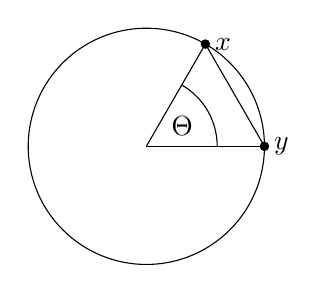
\begin{tikzpicture}[scale=1.5]
	\draw (0,0) circle (1);
	\draw (0,0)--(1,0) node[right]{$y$};
	\draw (0,0)--(60:1) node[right]{$x$};
	\draw (60:1)--(1,0);
	\draw (30:0.35) node{$\Theta$};
	\draw (0.6,0) arc [start angle=0, end angle=60, radius=0.6];
	\filldraw (1,0) circle (1pt);
	\filldraw (60:1) circle (1pt);
	\end{tikzpicture}
	
	\end{centering}

	With the statement of the theorem we get
	\[
	a(X,d)=\int_Xd(x,y)\mu_0(\dx)=\frac{1}{2\pi}\int_0^{2\pi}\sin\left(\frac{\Theta}{2}\right)\mathrm{d}\Theta=\frac{2}{\pi}.\]
\end{example}
This result can also be obtained by approximating the circle by regular $n$-gons with $n\to \infty$, see for example \cite{cleary:numbers-of-shapes} by Cleary, Morris and Yost. In Appendix \autoref{sourcecode} this is exemplified with a short Python3 script, which calculates the rendezvous value for $n$-gons of unit diameter as well as the error. 

The following lemma extend the result of the previous theorem and is also due to Morris and Nickolas \cite{Morris1983}.
\begin{lemma}
	Let $(X,d)$ be a compact, connected, non-empty %das fehlt in der quelle
	 metric space and let $\mu_0\in \M^1(X)$. If for each pair of points $y$ and $e$ in $X$ there exists an isometry $T: X\to X$ such that $T(y)=e$ and $\mu_0(A)=\mu_0(T(A))$ for all Borel sets $A$, then $\int_Xd(x,y)\mu_0(\dx)$ is independent of $y$.
\end{lemma}
\begin{proof}
	Let $y,e\in X$ and let $T$ be an isometry as described above. Then
	\begin{align*}
		\int_X d(x,y)\mu_0(dx)=&\int_X d(T(x),T(y))\mu_0(\dx)
		\\
		=&\int_Xd(T(x),e)\mu_0(\dx)
		\\
		=&\int_Xd(x,e)\mu_0(\mathrm{d}T^{-1}x)
		\\
		=&\int_Xd(x,e)\mu_0(\dx).
	\end{align*}
	Since there exists such $T$ for all pairs $y,e$ the expression above does not depend on $y$.
\end{proof}



\begin{corollary}
	Let $S^n$ be the $n$-dimensional sphere in $\R^{n+1}$, and let $d$ be the inherited metric on $S^n$. Let $\mu_0$ be the normalized Lebesgue measure on $S^n$. Then
	\[
	a(S^n,d)=\int_{S^n}d(x,y)\mu_0(\dx)
	\]
	for any $y\in S^n$.
\end{corollary}

According to Morris and Nickolas, this integral can be expressed as follows: Let $S^n$ be the $n$-sphere with radius $\frac{1}{2}$ then
\[
a(S^n,d)=\frac{2^n\left[\Gamma\left(\frac{n+1}{2}\right)\right]^2}{\sqrt{\pi}\Gamma\left(\frac{2n+1}{2}\right)}.
\]
The detailed computation was displayed by Chad \cite{chad}.
